\documentclass[a4paper,11pt]{article}
\usepackage[T1]{fontenc}
\usepackage[utf8]{inputenc}
\usepackage{lmodern}
\usepackage{graphicx}
\usepackage[german]{babel}
\usepackage{float}

\title{B-Tag 2015}
\author{Andreas Gwilt, Josua Brandhofer, Niclas Reichel, Thomas Mersch}

\begin{document}

\maketitle
\tableofcontents

\section{Aufgaben}
\subsection{Aufgabe 1: Dreiecksgeometrie}
\textbf{Ist $\overline{FE}$ länger als $\overline{CA}$?} \\

\begin{figure}[htbp] 
        \centering
        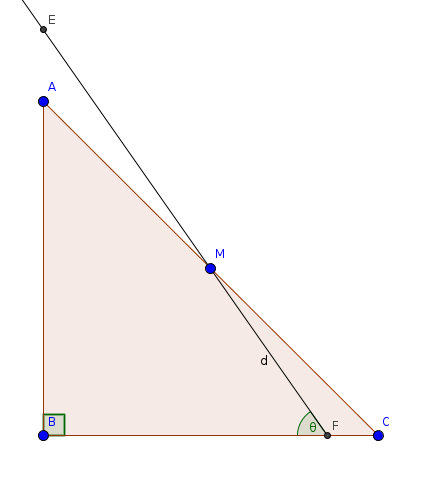
\includegraphics[width=6cm]{img/A1_1.png}
\end{figure}

Wir wollen eine Funktion $\overline{FE}(\theta)$ aufstellen, und zeigen, dass diese immer gr\"o\ss er als $\overline{CA}$ ist.

1. Wie lang ist die Strecke $\overline{FM}$?
\[ \overline{FM}(\theta) = \frac{M_y}{sin(\theta)} \]

2. Wie lang ist die Strecke $\overline{ME}$?
\[ \overline{ME}(\theta) = \frac{M_x}{sin((\pi/2)-\theta)} \]

3. Die Strecke $\overline{FE}$ ist also $\overline{FM} + \overline{ME}$ (natürlich alles im Definitionsbereich $0 < \theta < \frac{\pi}{2}$:
\[ \overline{FE}(\theta) = \frac{M_y}{\sin(\theta)} + \frac{M_x}{\sin((\pi/2)-\theta)} \]

Jetzt muss gezeigt werden, dass der Tiefpunkt von $\overline{FE}(\theta)$ den Wert $\overline{AC}$ hat. Dazu wird $\overline{FE}(\theta)$ zuerst abgeleitet, um den TP zu finden:

\[ \overline{FE}'(\theta) = \frac{M_x (\sin(\theta))^3 - M_y (\cos(\theta))^3)}{(\sin(\theta))^2 (\cos(\theta))^2} \]

Jetzt setzen wir $\overline{FE}' = 0$, um den Tiefpunkt von $\overline{FE}(\theta)$ bei $\theta = \frac{\pi}{4}$ zu finden, und sehen, dass $FE(\frac{\pi}{4}) = CA$ ist. Daher ist $\overline{FE}$ immer länger als $\overline{CA}$ (au\ss er bei $\theta=\frac{\pi}{2}$).

\subsection{Aufgabe 2: Verschiebungen}

\begin{figure}[htbp] 
        \centering
        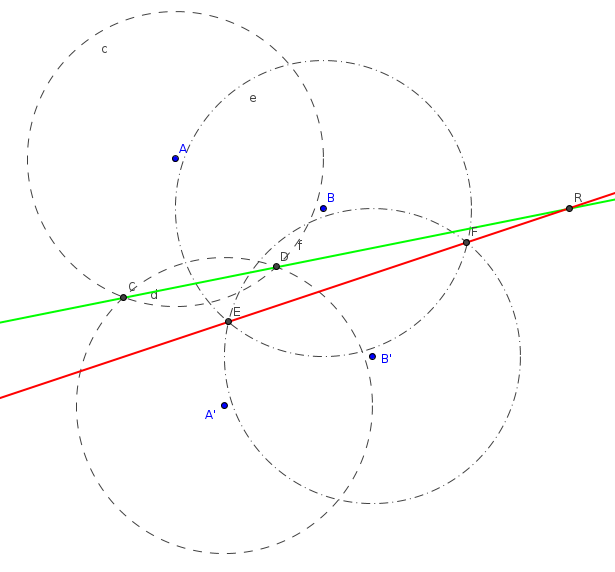
\includegraphics[width=8cm]{img/A2_1.png}
\end{figure}

\textbf{Wo ist das Drehzentrum R?} \\
Die Aufgabenstellung verlangte die Bestimmung eines Drehzentrums anhand 2 identischer, jedoch in der Lage 
veränderten Figuren, anhand zwei sich auf den Figuren befindenden Punkten. Zuerst machten wir uns folgende Bedingungen zu Nutze:

\[ |AR| = |A'R| \]
\[ |BR| = |B'R| \]

Wenn man nun um die verschobenen Punkte A und A' jeweils einen Kreis mit gleichem Radius legt, welcher so gewählt wird, sodass sich die Kreise schneiden.\\
Entlang der beiden Schnittpunkte lässt sich eine Gerade legen. Ebenso verfährt man mit Punkt B bzw. B'. \\
Das Drehzentrum R befindet sich im Schnittpunkt der beiden Geraden.

\subsection{Aufgabe 3: St\"ocke}

\begin{figure}[htbp] 
        \centering
        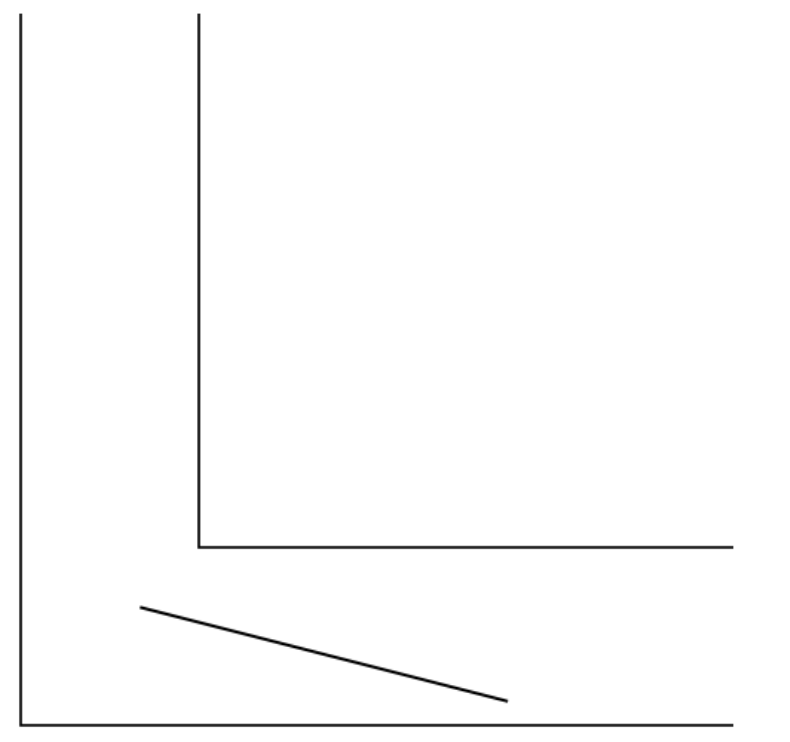
\includegraphics[width=6cm]{img/A3_1.png}
\end{figure}

\textbf{Welche St\"ocke passen auf jeden Fall nicht durch?} (Angenommen, der Gang ist 1 breit) \\
Die Stelle, an der die maximale Länge am kleinsten ist, ist wenn der Stock in einem $\frac{\pi}{4}$ Winkel zu den Wänden steht. Deshalb darf ein Stock auf jeden Fall nicht länger als die Diagonale an dieser Stelle sein, also $2\sqrt{2}$.

\textbf{Passt der $2\sqrt{2}$ Stock durch den Gang?} \\
Wir nehmen an, der Stock berührt die ganze zeit die innere Ecke (damit er durch passt). Dann haben wir die Gleiche Situation wie in A1. Die maximale Länge des Stocks wird immer größer, je weiter die Winkel zu den Wänden von $\frac{\pi}{4}$ sind. Deshalb passt ein Stock bei jedem Winkel, wenn er auch bei $\frac{\pi}{4}$ passt.

\subsection{Aufgabe 4: Strategien f\"ur den l\"angsten Stock}
\textbf{Wie muss das Drehzentrum R gew\"ahlt werden, damit der l\"angstm\"oglichste Stock in einer einzigen Drehbewegung um die Ecke bewegt werden kann?} \\

\begin{figure}[htbp] 
        \centering
        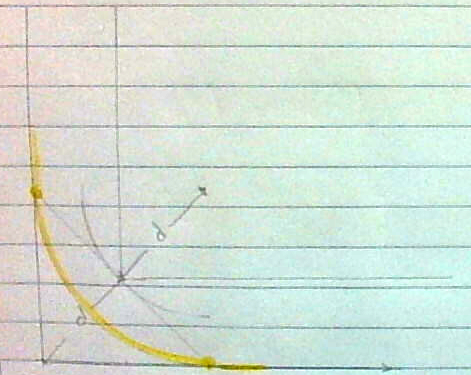
\includegraphics[width=6cm]{img/A4_1.png}
\end{figure}

Die Stockenden verlaufen auf einer kreisförmigen Schiene mit dem Radius $2d$. \\
d wird definiert als:

\[ d = \sqrt{B^2+B^2} \]

B beschreibt die Breite des Ganges. \\
Legt man nun ein Rechteck mit der Seitenlänge 2B in die Ecke des Ganges, befindet sich das Drehzentrum R an der gegenüberliegenden Spitze des Rechtecks. \\
Der Stock beginnt seine Drehung, welche am \"au\ss eren Rand beginnt, sobald er sich unterhalb des Drehzentrums R befindet.

Die Folgende Fl\"ache wird also \"uberstrichen:
\begin{figure}[htbp] 
        \centering
        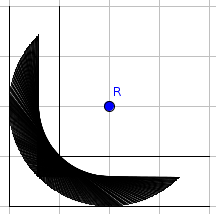
\includegraphics[width=4cm]{img/A4_2.png}
\end{figure}

\textbf{Bei einer anderen M\"oglichkeit bleiben die Enden des Stocks st\"andig mit den Au\ss enw\"anden des Ganges in Kontakt.} \\
Dabei beschreibt folgende Kurve die Bewegung vom Mittelpunkt des Stocks:
\begin{figure}[H] 
        \centering
        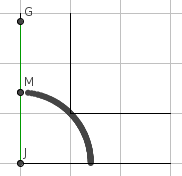
\includegraphics[width=4cm]{img/A4_3.png}
\end{figure}

Und hier die vom Stock \"uberstrichene Fl\"ache:
\begin{figure}[H] 
        \centering
        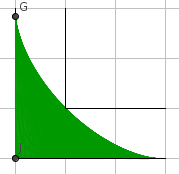
\includegraphics[width=4cm]{img/A4_4.png}
\end{figure}

\subsection{Aufgabe 5: Gr\"o\ss te Rechtecke}

\textbf{Wie groß ist der Flächeninhalt des größten Rechtecks, das um die Ecke bewegt werden kann,
wenn die kürzere Seite des Rechtecks die Länge 0,5 hat?} \\
Wenn die H\"ohe des Rechtecks 0.5 ist, ist die gr\"o\ss te Breite 1. Dann hat man eine Fl\"ache von 0.5.
Wenn die Breite 0.5 ist, muss erst einmal ausgerechnet werden, was die maximale H\"ohe ist. Das Rechteck muss im Winkel von $\frac{\pi}{4}$ noch passen: 

\begin{figure}[htbp] 
        \centering
        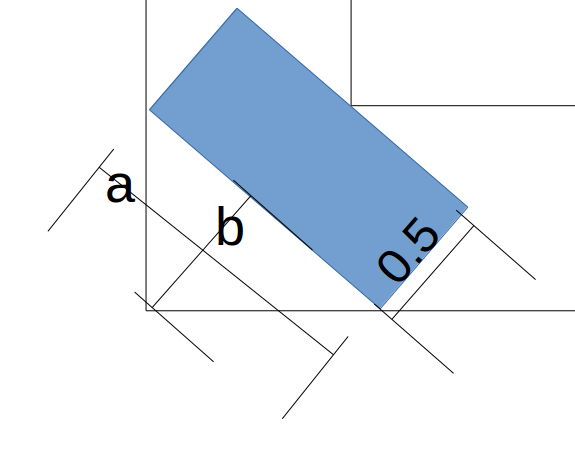
\includegraphics[width=6cm]{img/A5_1.png}
\end{figure}

\[ s = \sqrt{2} - 0.5 \]
\[ s = \frac{a}{2} \Leftrightarrow a = 2s = 2(\sqrt{2}-0.5) \]

$a$ w\"are also in dem Fall ca. 1.83, was einen Fl\"acheninhalt von ca. 0.914 ergibt.

\textbf{Welche Seitenl\"angen hat das Rechteck mit dem gr\"o\ss ten Fl\"acheninhalt, was noch durch den Gang passt, wobei die k\"urzere Seite nicht \"uber 0.5 ist?} \\
Allgemeine Formel f\"ur das Maximale $a$ mit einer festgesetzten seitenl\"ange b:

\[ a = 2(\sqrt{2}-b) \]

Daraus kann man eine Funktion der maximalen Fl\"ache $A_{max}(b)$ des rechtecks $a \times b$ konstruieren:

\[ A_{max}(b) = a b = 2c(\sqrt{2}-b) \]

\begin{figure}[htbp] 
        \centering
        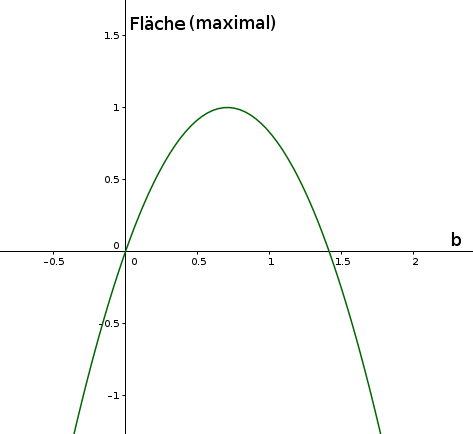
\includegraphics[width=6cm]{img/A5_2.png}
\end{figure}

Man kann einfach ablesen, dass die kurze Seite nicht unter 0.5 sein sollte. Daher wird das selbe Rechteck wie vorhin gesucht:

\[ b = 0.5 \]
\[ a = 2(\sqrt{2}-b) \approx 1.83 \]

Hier ist das Rechteck bei der engsten Stelle: (ab dieser Stelle passt es natürlich locker, (siehe A1))

\begin{figure}[htbp] 
        \centering
        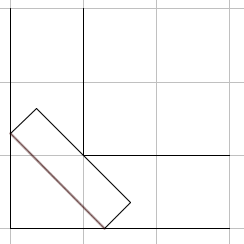
\includegraphics[width=6cm]{img/A5_3.png}
\end{figure}

\subsection{Aufgabe 6: Alle Rechtecke}

\subsection{Aufgabe 7: U-Form}
\begin{figure}[H] 
        \centering
        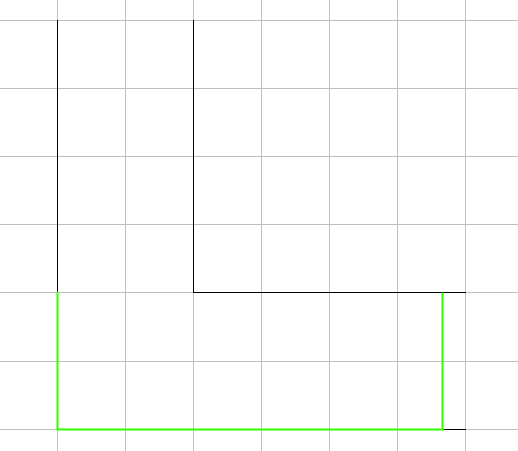
\includegraphics[width=5cm]{img/A7_1.png}
        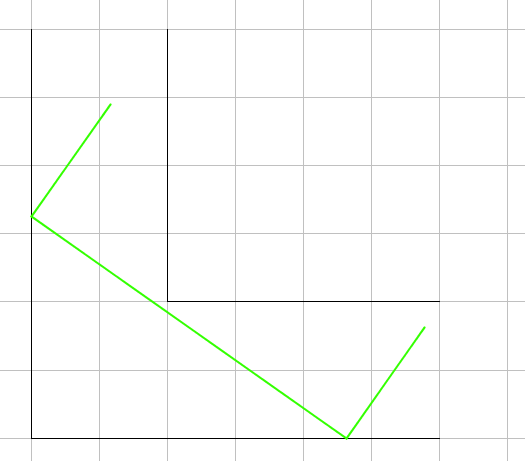
\includegraphics[width=5cm]{img/A7_2.png}
\end{figure}
In den vorherigen Aufgaben wurde bereits die maximale Länge eines Stockes, welcher um die Ecke passt herausgefunden. Nun werden wir an diesen 2 weitere Stöcke befestigen, sodass eine U-Form entsteht und er immernoch um die Ecke passt. Die maximale Länge der 2 neuen Stöcke ist von der “engsten” Stelle abhängig, welche sich vor dem Beginn der Drehung befindet.\\

Somit ist die Breite des Ganges äquivalent zur maximalen Länge der neuen Stöcke und die Gesamtlänge des großtmöglichsten u-förmigen Stockes die zweifache Breite des Ganges addiert mit der zuvor bestimmten Maximallänge des “Hauptstockes”.

\[ L_{max} = 2(b+\sqrt{b^2+b^2}) \]

Eingesetzt:

\[ 2(1+\sqrt{2})=4.83 \]

\subsection{Aufgabe 8: L-Form}
\textbf{Was ist die l\"angste (a+b) L Form, die durch den Gang passt?} \\

\begin{figure}[htbp] 
        \centering
        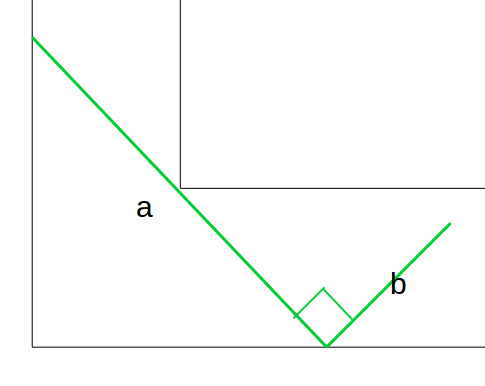
\includegraphics[width=6cm]{img/A8_1.png}
\end{figure}

Die kürzere Seite ($b$) darf natürlich nicht länger als 1 sein, sonst passt das ganze L nicht durch den Gang. \\
Auch darf $a$ nicht \"uber $2\sqrt{2}$ sein, sonst passt die ganze Form schräg gestellt in die Ecke. \\
Eine solche L-Form ($1+2\sqrt{2}$) müsste auch durch passen: Die lange Seite kann so durch geschoben werden, dass die Enden immer die Außenwand berühren. Die kurze passt dann auch, da sie immer die Außenwand mit einem Ende berührt und im ``schlimmsten'' fall die Innenwand mit dem anderen berührt.

\section{Forschungsauftrag}
\textbf{Was ist das größte Ding, was durchgejagt werden kann?}

\subsection{Rechteck}
Was ist das größte Rechteck, was man durch den Gang schieben kann? Ohne drehen ist es natürlich ein $1\times 1$ Quadrat. Mit drehen ist wieder die Funktion $A_{max}(b)$ hilfreich. Sie beschreibt das Rechteck der größten Fläche was noch durch passt, abhängig von einer festen kürzeren Seitenlänge $b$:

\[ A_{max}(b) = 2b(\sqrt{2}-b) \]

\begin{figure}[htbp] 
        \centering
        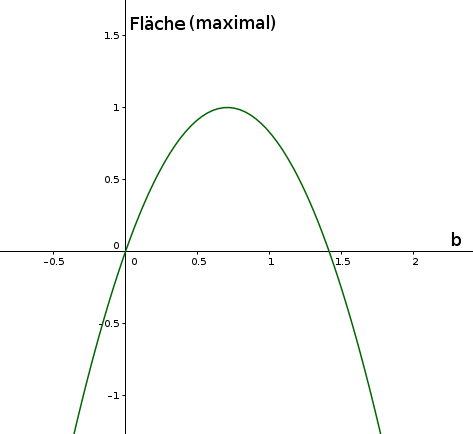
\includegraphics[width=6cm]{img/FA_1.png}
\end{figure}

Diese Funktion beschreibt also alle größten Rechtecke, die durch schieben \textit{und} drehen durch passen. Dabei ist der Hochpunkt das größtmögliche Rechteck. Um den Hochpunkt zu finden leiten wir zuerst ab:

\[ A_{max}'(b) = 2(\sqrt{2}-2b) \]

Um dann davon die Nullstelle bei $b = \frac{1}{\sqrt{2}}$ zu finden. Hier ist das größte Rechteck, mit einer Fläche von

\[ A_{max}(\frac{1}{\sqrt{2}}) = \frac{2}{\sqrt{2}}(\sqrt{2} - \frac{1}{\sqrt{2}}) = 1 \]

also erstaunlicherweise der gleiche Inhalt wie ein $1\times 1$ quadrat. Ein Rechteck mit demg Flächeninhalt > 1 kann also einfach nicht durch den Gang geschoben werden, egal ob quadratisch oder nicht.

\end{document}
